
%----------------------------------------------------------------------------------------
%	PREAMBUŁA
%----------------------------------------------------------------------------------------

\documentclass[11pt]{article}
\usepackage[polish]{babel}
\usepackage{polski}
\usepackage[utf8]{inputenc}
%\usepackage[T1]{fontenc}
\usepackage{amsmath}
\usepackage{graphicx}
\usepackage{fancyhdr}
\usepackage{float}
\usepackage{graphicx}
\usepackage{hyperref}
\usepackage{verbatim}

\usepackage{subfig}


\usepackage{color} %red, green, blue, yellow, cyan, magenta, black, white
\definecolor{mygreen}{RGB}{28,172,0} % color values Red, Green, Blue
\definecolor{mylilas}{RGB}{170,55,241}

%\usepackage{ucs}
%\usepackage{lmodern}
\usepackage{listings}

% Polskie literki w listingach:
\lstset{   
    texcl=true,
    inputencoding=utf8,
    extendedchars=true,
    literate=
    {ą}{{\k{a}}}1 {Ą}{{\k{A}}}1 
    {ł}{{\l{}}}1 {Ł}{{\L{}}}1 
    {ń}{{\'n}}1 {Ń}{{\'N}}1 
    {ę}{{\k{e}}}1 {Ę}{{\k{E}}}1 
    {ś}{{\'s}}1 {Ś}{{\'S}}1 
    {ż}{{\.z}}1 {Ż}{{\.Z}}1 
    {ó}{{\'o}}1 {Ó}{{\'O}}1 
    {ź}{{\'z}}1 {Ź}{{\'Z}}1 
    {ć}{{\'c}}1 {Ć}{{\'C}}1
}

\lstset{language=Matlab,%
    %basicstyle=\color{red},
    breaklines=true,%
    morekeywords={matlab2tikz},
    keywordstyle=\color{blue},%
    morekeywords=[2]{1}, keywordstyle=[2]{\color{black}},
    identifierstyle=\color{black},%
    stringstyle=\color{mylilas},
    commentstyle=\color{mygreen},%
    showstringspaces=false,%without this there will be a symbol in the places where there is a space
    numbers=left,%
    numberstyle={\tiny \color{black}},% size of the numbers
    numbersep=9pt, % this defines how far the numbers are from the text
    emph=[1]{for,end,break},emphstyle=[1]\color{red} %some words to emphasise
    %emph=[2]{word1,word2}, emphstyle=[2]{style}, 
}


\title{Sprawozdanie}
\author{Aleksandra Poręba}

\graphicspath{{static/}{../images/}} 

\makeatletter
\let\thetitle\@title
\let\theauthor\@author
\let\thedate\@date
\makeatother


%----------------------------------------------------------------------------------------
%	STRONA TYTUŁOWA
%----------------------------------------------------------------------------------------
\begin{document}
\begin{center}
\textsc{\normalsize Wydział Fizyki i Informatyki Stosowanej}\\[2.0cm] 

\includegraphics[scale = 1]{logo.png}\\[1cm] 
%\textsc{\Large Modelowanie Procesów Fizycznych}\\[0.4cm] 


\textsc{\Large Sprawozdanie}\\[0.4cm]
{ \huge \bfseries \LARGE{Algorytmy Genetyczne - Projekt} }\\[1cm] 

\flushright \Large Aleksandra Poręba \\ nr. indeksu 290514

\vfill 

\center{\today}


\pagebreak 

\end{center}

%----------------------------------------------------------------------------------------
%	SPIS TREŚCI
%----------------------------------------------------------------------------------------
%\tableofcontents
%\pagebreak

%----------------------------------------------------------------------------------------
%	ZAWARTOŚĆ
%----------------------------------------------------------------------------------------

\pagestyle{fancy}
\fancyhf{}

\rhead{\theauthor}
\lhead{\thetitle}
\cfoot{\thepage}

\section{Wstęp}
Celem projektu było napisanie programu znajdującego lokalizację małych płytek na dużej płycie, tak, aby powierzchnia małych płytek była jak największa. Do rozwiązania tego problemu został napisany program wykorzystujący algorytm genetyczny.

Jako dane wejściowe program przyjmuje listę wymiarów małych płyt. Powinna być ona zapisana w pliku $maleplyty.txt$, znajdującym się w tym samym katalogu, co plik wykonywalny programu. Wartości powinny zostać podane w milimetrach. Wymiary dużej płyty są z góry znane i wynoszą $2800x2070 [mm]$.

Jako wyjście program zapisuje do pliku $output.txt$ pole rozplanowanych płytek, oraz kolejno:
\begin{itemize}
\item szerokość i wysokość płytki,
\item współrzędne lewego górnego rogu płytki - jeśli nie zostanie ona wycięta wartości te będą równe $-1$,
\item flaga, czy płytka ma zostać obrócona przy cięciu.
\end{itemize}

Do napisania programu został wykorzystany język $C++$ wraz z biblioteką $GALib$ oraz język \textit{python + turtle} do rysowania rozkładu płytek.

\section{Algorytm i kodowanie}
W algorytmie, po przeprowadzeniu testów, ustawiono 600 pokoleń oraz 1000 osobników. Została włączona również opcja gwarantująca nie ujemność funkcji dostosowania - gdy kary są wyjątkowo wysokie, może przyjmować ona ujemne wartości.

W programie zostało wykorzystane kodowanie rzeczywistoliczbowe, z wartościami całkowitymi. Za lokalizacje jednej płytki odpowiada czwórka: \textit{położenie lewego górnego wierzchołka (x, y), czy płytka jest obrócona, czy płytka ma zostać wycięta}.

Dane te mogą przyjmować następujące wartości:
\begin{itemize}
\item $ 0 \leq x \leq 2800$,
\item $ 0 \leq y \leq 2070$,
\item $ r \in \{0, 1\} $,
\item $ e \in \{0, 1\}$.
\end{itemize}

Dzięki takiemu kodowaniu wartości, zgodnie z założeniami, będą całkowite oraz w zadanych obszarach.

\section{Funkcja dostosowania}
Funkcja dostosowania algorytmu została przedstawiona w następujący sposób:
\begin{equation}
f(S_i) = \sum_j P_{i, j} - a \cdot g(S_i) - b \cdot  h(S_i)
\end{equation}
\begin{description}
\item $S_i$ - położenia płytek dla danego genomu,
\item $P_{i, j}$ - pole $j$-tej płytki,
\item $a$ - parametr skalujący funkcję kary $g$,
\item $g(S_i)$ - funkcja kary wychodzenia poza obszar dużej płyty,
\item $b$ - parametr skalujący funkcję kary $h$,
\item $h(S_i)$ - funkcja kary przecinania się z innymi płytkami.
\end{description}

Funkcja kary sprawdzająca wychodzenie poza wyznaczony obszar uruchamiana jest dla każdej płytki. Zwraca ona kwadrat pola, które ''wystaje'' poza dużą płytę.

Kara za przecięcie z innymi płytkami obliczana jest dla każdej pary płytek. Liczone jest pole wspólnego obszaru obu kształtów, funkcja kary zwraca kwadrat tej wartości.

W trakcie ewolucji parametry kary aktualizowane są trzykrotnie. Na samym początku wartości $a, b = 10$, po upływie $180$ pokoleń ($0.3$ ustawionej liczby pokoleń) wartość ta jest zwiększana do $100$, a następnie, po kolejnych $120$ pokoleniach do $1000$. Zwiększając te współczynniki stopniowo algorytm eliminuje słabe, nieprawidłowe rozwiązania jednocześnie nie odrzucając rozwiązań bardzo dobrych, ale z małym błędem i pozwala im wyewoluować w dobrym kierunku. 

W ostatniej aktualizacji, po $0.7$ liczby wszystkich pokoleń wyłączane jest karanie w funkcji dostosowania, tak, aby ostatecznie uzyskać jedynie poprawne wyniki. Wtedy, w przypadku przecięcia, funkcja dostosowania jest zerowana.

\section{Testowanie parametrów}
W algorytmie została włączona sukcesja elitarna, dzięki której algorytm uzyskiwał lepsze wyniki. Podobnie jak w przypadku zadania z laboratorium 7 zmiany przy operatorze krzyżowania nie wpływały znacząco na otrzymywane wyniki, więc pozostawiono domyślny operator, a jego prawdopodobieństwo ustawione zostało na wartość $0.3$.

Zostały przetestowane następujące operatory selekcji:
\begin{itemize}
\item selekcja ruletkowa,
\item selekcja deterministyczna,
\item selekcja rankingowa,
\item selekcja turniejowa.
\end{itemize}

Prawdopodobieństwo mutacji zostało ustawione na $0.05$. Uzyskane wyniki dla 30 testów zostały przedstawione poniżej.

\begin{figure}[H]
\centering
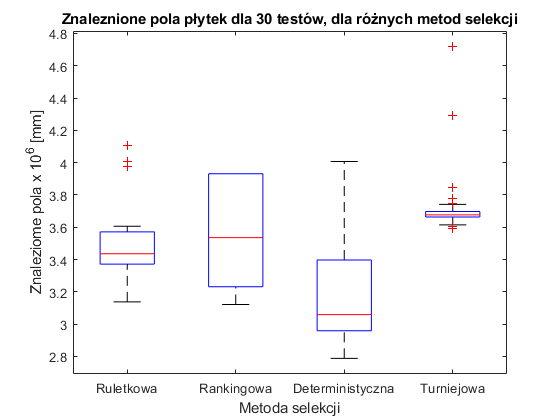
\includegraphics[width=0.6\textwidth]{test_selekcja.png}
\caption{Wyniki 30 testów różnych parametrów, przedstawione w formie wykresu \textit{pudełka z wąsami}. Najlepsze wyniki osiągała selekcja turniejowa, najgorsze deterministyczna. }
\end{figure}

Jako najlepsza została wybrana selekcja turniejowa - uzyskujemy dla niej najwyższe wartości pola małych płytek. Średnie wyniki które osiąga skoncentrowane w okolicach $3.7 * 10^6$.  Algorytm genetyczny jest uruchamiany wiele razy w czasie pojedynczego uruchomienia programu, więc możemy się spodziewać, że uda się mu odnaleźć wartości odstające, które dla tej selekcji są najwyższe.

Dla wybranej selekcji przetestowano różne wartości prawdopodobieństwa mutacji.

\begin{figure}[H]
\centering
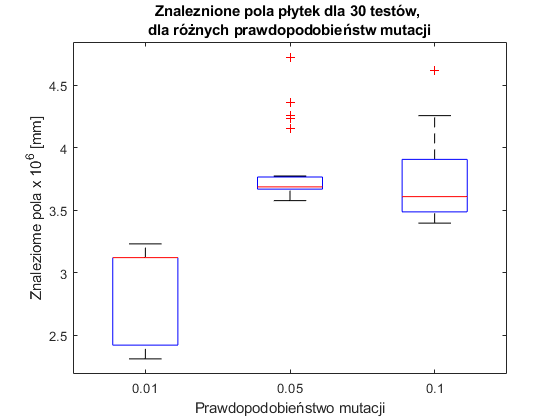
\includegraphics[width=0.6\textwidth]{test_mutacja.png}
\caption{Wyniki 30 testów różnych parametrów, przedstawione w formie wykresu \textit{pudełka z wąsami}. Zadowalające wyniki osiągały wartości $0.05$ oraz $0.1$. }
\end{figure}

Finalnie została wybrana wartość $p_m = 0.05$.

\section{Uruchomienie programu}
Aby uruchomić skompilowaną wersję programu należy uruchomić plik $AG\_proj.exe$ znajdujący się w katalogu $exe$. Plik wejściowy o nazwie $maleplyty.txt$ powinien znajdować się w tym samym katalogu.

Jako wynik działania tworzony jest plik $output.txt$, w którym znajduje się suma pól małych płyt, które zostaną wycięte, ich położenia - zgodnie z zadanym formatem. Ten plik może zostać użyty do uruchomienia skryptu $draw_results.py$, który przedstawi wycięcie płytek w sposób graficzny. Aby użyć programu konieczne jest włączenie opcji przekazywania sesji $X11$. 

Skrypt do rysowania kolejno zaprezentuje ustawienie płytek, tak jakby były wycinane. Aby wyjść z programu po zakończeniu rysowania należy kliknąć w okno. Wynik zostanie zapisany do pliku $board.eps$. Przykładowy wynik został przedstawiony poniżej.

\begin{figure}[H]
\centering
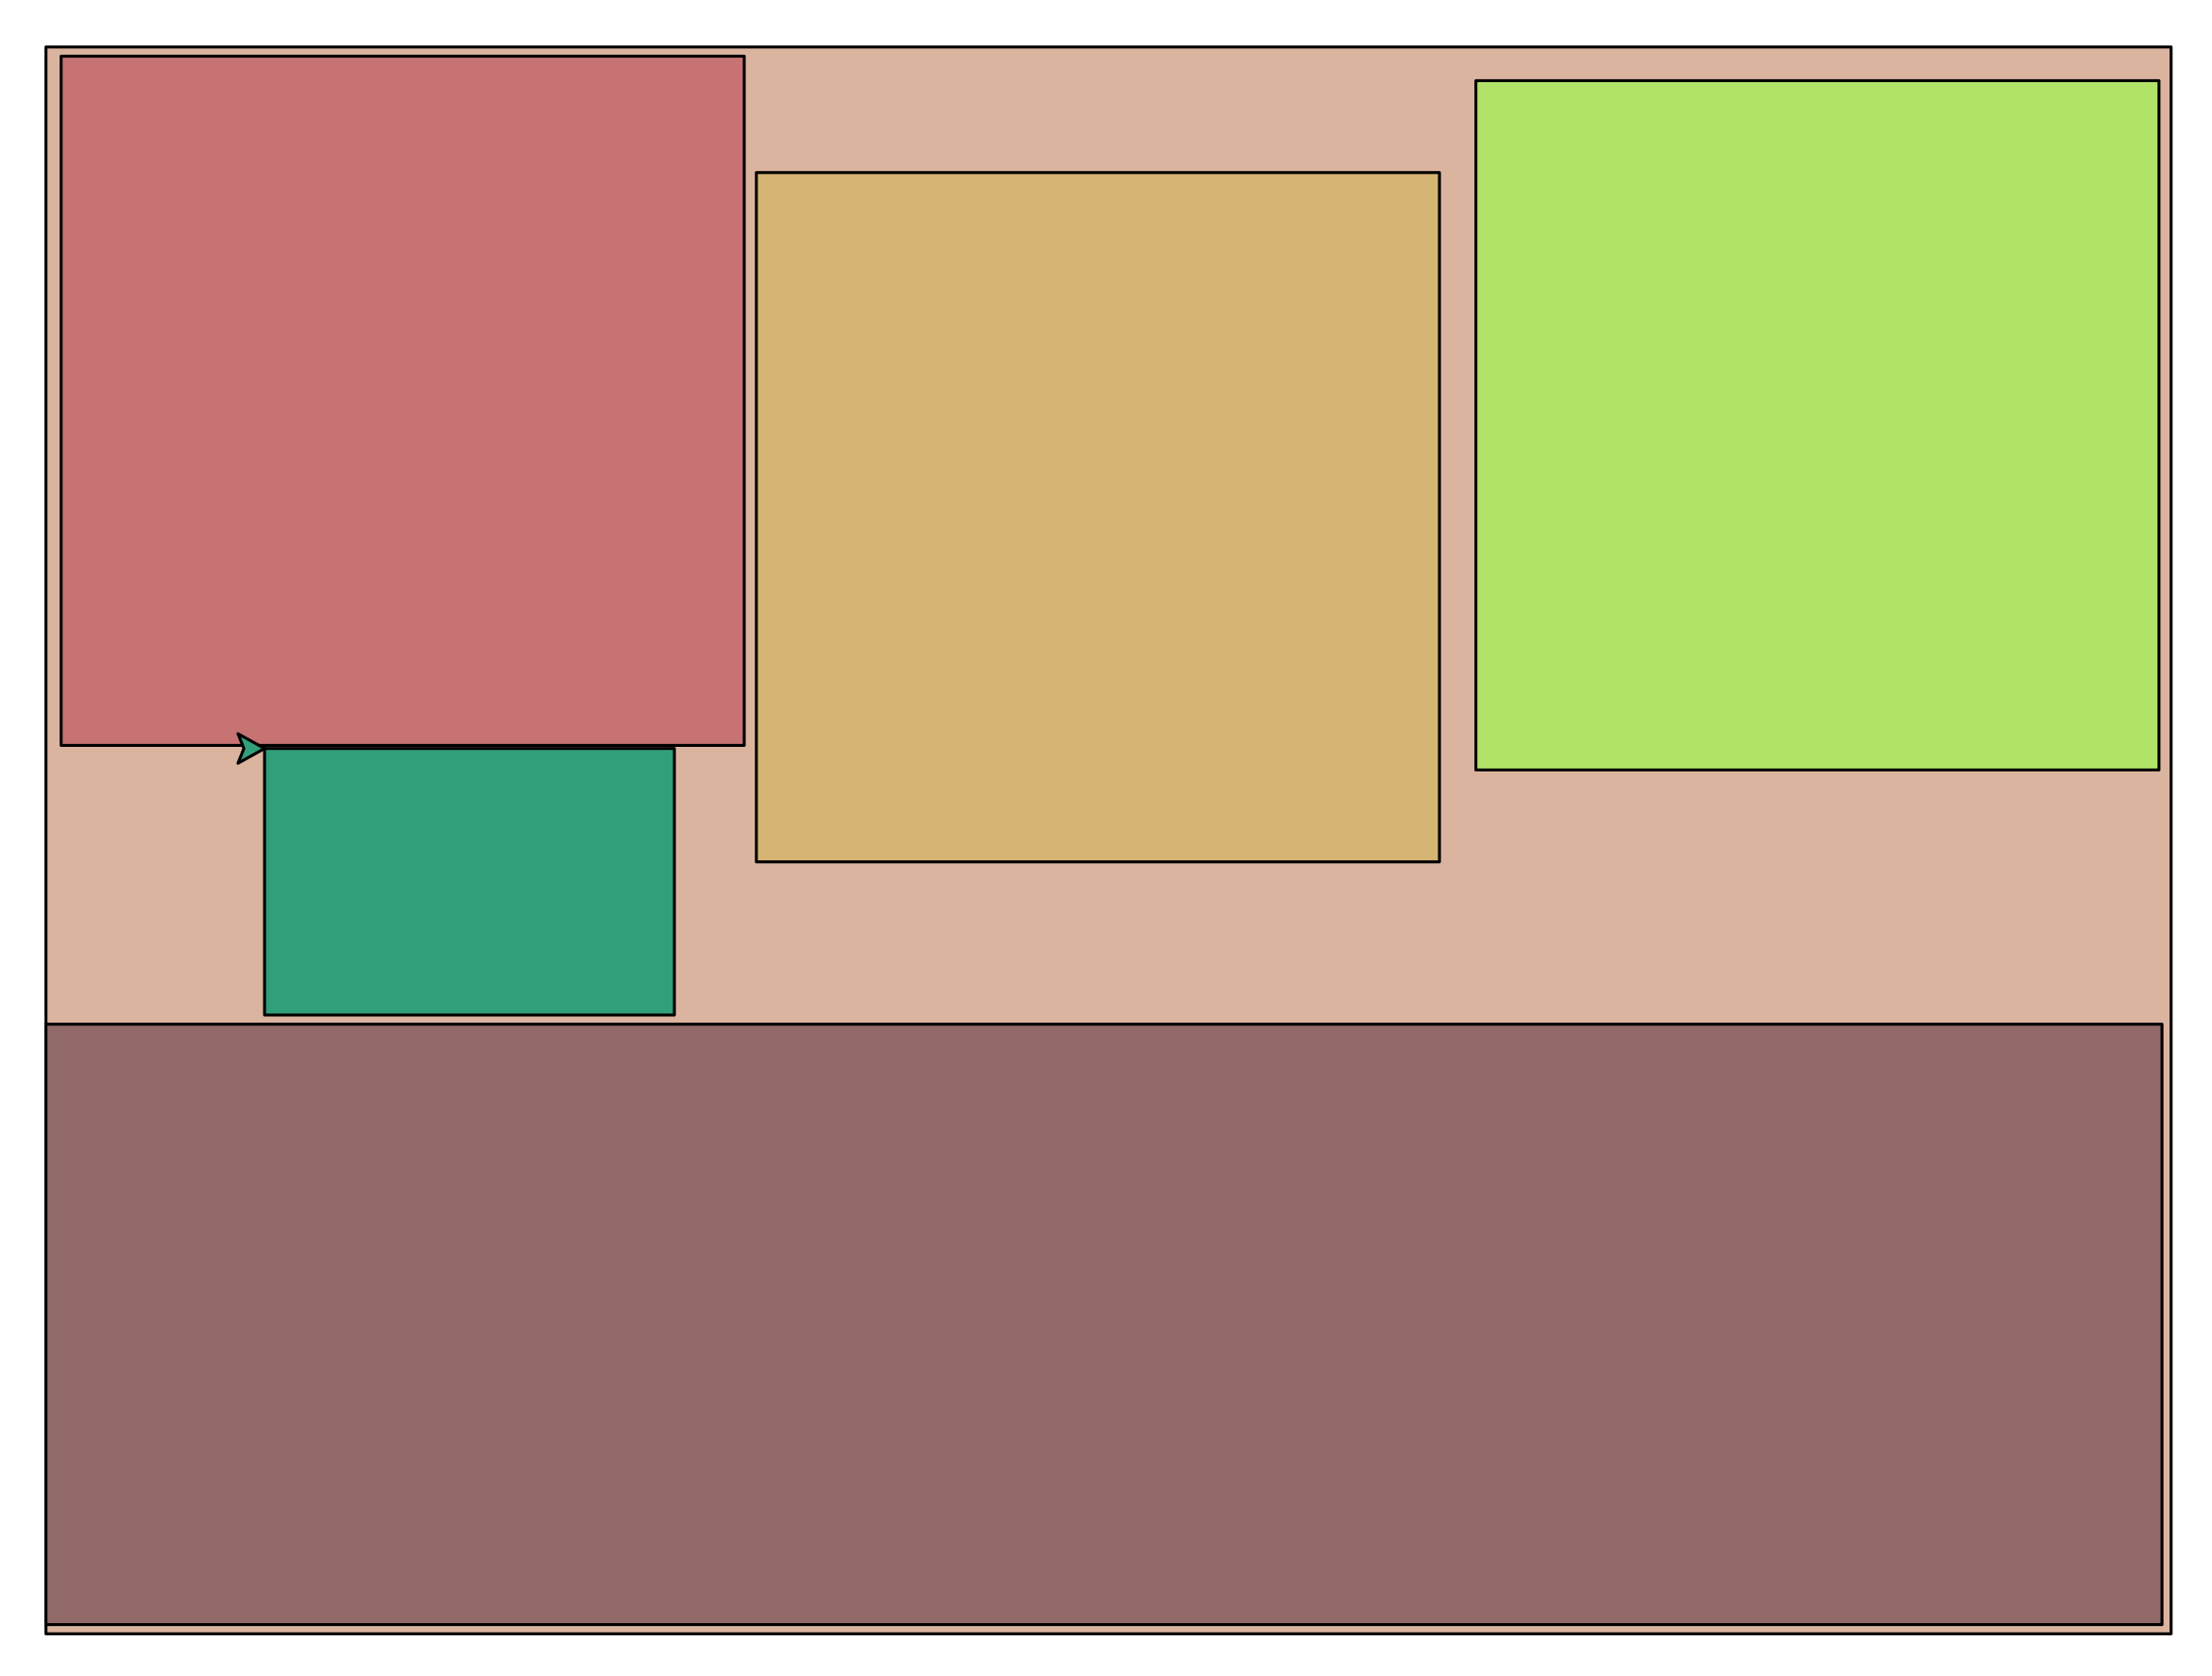
\includegraphics[width=0.6\textwidth]{board.png}
\caption{Graficzna reprezentacja przykładowego rozkładu płytek, dla pola równego $4.81 * 10^6$}
\end{figure}

Aby skompilować program można użyć narzędzia $cmake$ i wykorzystać przygotowany plik $CMakeLists.txt$. Znajduje się on w katalogu $AG$. Wymagane jest posiadanie biblioteki $GALib$.

\vspace{0.5cm}

Została przetestowana poprawność działania funkcji obliczającej karę dla różnych położeń płytek. Przygotowany test znajduje się w katalogu $test$. Aby go uruchomić również można skorzystać z przygotowanego pliku $CMakeLists.txt$, tym razem z katalogu $test$. Testy sprawdzają, czy jest poprawnie obliczane pole przecięcia płytek, oraz czy płytka nie wystaje poza wyznaczony obszar.

\end{document}

